
\documentclass[12pt]{article}

\usepackage{algpseudocode}
\usepackage{amsfonts}
\usepackage{amsmath}
\usepackage{amssymb}
\usepackage[backend=bibtex]{biblatex}
\usepackage{color}
\usepackage{fullpage}
%\usepackage{geometry}
\usepackage{mathrsfs}
\usepackage{mathtools}
\usepackage{parskip}
\usepackage{tikz}

\addbibresource{tp.bib}

\newcommand{\ds}{\displaystyle}

\begin{document}

\title{Truncatable Primes - Statistics and Estimations}
\author{TKoz}
\date{\today}
\maketitle

\begin{abstract}
Not written yet.
\end{abstract}

\section{Introduction}

In number theory, truncatable primes are prime numbers such that some of their digits can be removed in succession, producing a sequence of primes until ending with, typically, a one digit prime. They can be defined for various number bases. In base 10, the number 2393 is a right truncatable prime because it is prime and we can remove a digit from the right one at a time to produce 239, 23, and 2, which are all prime. The number 1223 is a left truncatable prime because itself and 223, 23, and 3 are all prime.

The prime number theorem can be used to come up with a way to estimate how many truncatable primes there are in a given base, leading to the conjecture that there are finitely many in all bases for each of the types considered here. This can be proven for a specific base by computing all of them, but it has not been proven to be true for all bases.

\section{Definitions}

Note that all numbers are integers unless otherwise stated. In the following sections, basic definitions are given for some relevant mathematics used and then the four truncatable prime types considered are defined.

\subsection{Basics}

\textbf{Definition:} Euler's totient function, $\phi(n)$, defined for $n\geq1$, is how many numbers $1\leq x\leq n$ satisfy $\gcd(x,n)=1$.

\textbf{Definition:} The prime counting function, $\pi(n)$, defined for $n\geq1$, is how many prime numbers are $\leq n$.

\textbf{Definition:} A $d$ digit number ($d\geq1$) in base $b$ ($b\geq2$) can be expressed as:
$$ a_{d-1}b^{d-1} + a_{d-2}b^{d-2} + \ldots + a_1b^1 + a_0b^0 $$
Where $0<a_{d-1}<b$ and $0\leq a_i<b$ for $0\leq i\leq d-2$. The $a_i$ values are the digits of the number and their associated $b^i$ is the place value. The rightmost digit is $a_0$ and the leftmost digit is $a_{d-1}$. The number written in standard form in base $b$ is $(a_{d-1},a_{d-2},\ldots,a_1,a_0)$, written as an ordered tuple to differentiate from multiplication.

\subsection{Prime Types}

The truncatable prime types can be defined recursively. A number $n$ is a truncatable prime iff it is prime and its truncation (depending on the type) is also a truncatable prime. This produces a path of primes down to a base case.

\textbf{Right Truncatable:} Let $n=(a_{d-1},a_{d-2},\ldots,a_1,a_0)$ be a $d$ digit prime in base $b$. Then $n$ if a right truncatable prime iff $d=1$ or $(a_{d-1},a_{d-2},\ldots,a_2,a_1)$ is a right truncatable prime (equal to $\lfloor n/b\rfloor$, the rightmost digit is truncated).

\textbf{Left Truncatable:} Let $n=(a_{d-1},a_{d-2},\ldots,a_1,a_0)$ be a $d$ digit prime in base $b$. Then $n$ is a left truncatable prime iff $d=1$ or $(a_{d-2},a_{d-3},\ldots,a_1,a_0)$ is a left truncatable prime (equal to $n-a_{d-1}b^{d-1}$, the leftmost digit is truncated).

\textbf{Left-And-Right Truncatable:} Let $n=(a_{d-1},a_{d-2},\ldots,a_1,a_0)$ be a $d$ digit prime in base $b$. Then $n$ is a left-and-right truncatable prime iff $d=1$, $d=2$, or $(a_{d-2},a_{d-3},\ldots,a_2,a_1)$ is a left-and-right truncatable prime (equal to $\lfloor(n-a_{d-1}b^{d-1})/b\rfloor$, both the leftmost and rightmost digits are truncated).

\textbf{Left-Or-Right Truncatable:} Let $n=(a_{d-1},a_{d-2},\ldots,a_1,a_0)$ be a $d$ digit prime in base $b$. Then $n$ is a left-or-right truncatable prime iff $d=1$ or $(a_{d-2},a_{d-3},\ldots,a_1,a_0)$ is a left-or-right truncatable prime (left digit truncated) or $(a_{d-1},a_{d-2},\ldots,a_2,a_1)$ is a left-or-right truncatable prime (right digit truncated).

\section{Primality Testing}

Certifying primality would be prohibitively expensive for larger trees. In practice, the BPSW primality test does very well, and no BPSW pseudoprimes are known. The BPSW test combines a 2-SPRP test and a strong Lucas test with carefully chosen parameters. In practice, it should be extremely unlikely to encounter a BPSW pseudoprime so this primality test should be sufficient for getting very approximate or exact counts for how many truncatable primes there are of a particular type.

\section{Algorithms}

\subsection{Computing the Tree}

The recursive definitions of the truncatable prime types allows us to trace back to a 1 digit prime (or 2 digit for left-and-right truncatable). This is following a path up a tree toward its root. For the purpose of considering all truncatable primes of a particular type and base, we will let 0 be the root of the entire tree and have its child nodes be the base case primes. For example, in base 10, part of the right truncatable primes tree is:

\begin{center}
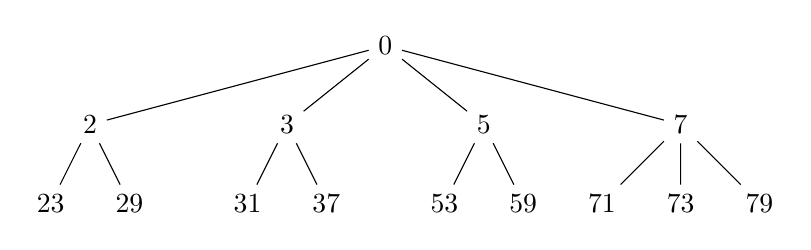
\begin{tikzpicture}
[
    level 2/.style = {sibling distance = 1cm}
]
\node {0} [sibling distance = 2.5cm, level distance = 1cm]
    child {
    node {2}
        child {node {23}}
        child {node {29}}
    }
    child {
    node {3}
        child {node {31}}
        child {node {37}}
    }
    child {
    node {5}
        child {node {53}}
        child {node {59}}
    }
    child {
    node {7}
        child {node {71}}
        child {node {73}}
        child {node {79}}
    };
\end{tikzpicture}
\end{center}

The tree can be explored using depth-first search which requires little memory since the tree height is expected to grow slowly. The recursion starts at a single digit prime and then tries every possible digit append to construct longer primes. The recursion is terminated at leaf nodes where it is not possible to append digits to construct a new prime. This method of searching exhaustively explores all possibilities.

For all truncatable prime types except left-or-right truncatable, each prime on the tree will have a unique path to the root by following the recursive definition. However, a left-or-right truncatable prime may have multiple paths and appear in the tree multiple times. For example, in base 10, the paths $3\to13\to313$ and $3\to31\to313$ are both valid paths to 313. Using depth-first search, 313 would be counted twice. For left-or-right truncatable primes, it is more appropriate to use breadth-first search to avoid duplicates, however this also requires more memory to store all the primes on a layer of the tree using a set data structure that eliminates duplicates. This also complicates parallelizing because separate subtrees may contain the same prime.

Finally, it is helpful to show that this method will actually find all the primes and nothing else. The base cases are small primes that satisfy the recursive definition of truncatable primes. Any further primes constructed recursively satisfy the definition because truncating the appended digits results in the smaller truncatable prime in its parent node. Conversely, for any prime satisfying the definition of a truncatable prime, we can construct a path of primes down to the base case. The recursive exploration of the tree will find this path in order of increasing digit length by exhaustively trying all possibilities. Therefore, ignoring duplicates for left-or-right truncatable primes, the set of numbers found recursively is the same as the set of all truncatable primes for any of the 4 types defined.

\subsection{Tree Hashing}

For the purpose of verifying computations, a hashing algorithm can be used. In order to allow computations to be split up and run in parallel, it makes sense to determine a hash for each node by combining its value with hashes of its children, using the root hash as the hash for the entire tree. A node in the tree with $k$ children may look like:

\begin{center}
\begin{tikzpicture}
\node {$r$} [sibling distance = 2.5cm, level distance = 2cm]
    child { node {$c_1$} edge from parent node [left] {$d_1$} }
    child { node {$c_2$} edge from parent node [left] {$d_2$} }
    child { node {$\ldots$} edge from parent [dashed] node {$\ldots$} }
    child { node {$c_k$} edge from parent node [left] {$d_k$} };
\end{tikzpicture}
\end{center}

Here, $r$ is the prime value in the node, $c_i$ are the child node hashes, and $d_i$ are the digit append values determined based on prime type and the digit(s) appended to create the child prime. The function $\text{irem}(n,d)$ is the remainder $r$ ($0\leq r<d$) of $n$ divided by $d$. The following algorithm is used to compute a 64 bit hash:

\begin{algorithmic}[1]
\Function{TreeNodeHash}{$r$,$d_i$,$c_i$}
\State $h \gets \lfloor \text{irem}(r,2^{64}) / 2 \rfloor$ \Comment{lowest 64 bits of $r$ shifted right 1: $r>>1$}
\For{$i=1$ to $k$}
\State $h' \gets \text{irem}(127h-d_i,2^{64})$
\State $h' \gets \text{irem}(8191h'+c_i,2^{64})$
\State $h' \gets \text{irem}(2^{19}h'+\lfloor h'/2^{45}\rfloor,2^{64})$ \Comment{rotate left 19 bits: $(h' << 19) | (h' >> 45)$}
\State $h \gets h \oplus h'$ \Comment{XOR with temporary value}
\EndFor
\State \Return $h$
\EndFunction
\end{algorithmic}

This combines some fast operations to compute a hash with decently random distribution. The multipliers 127 and 8191 are Mersenne primes chosen so multiplication can be computed with a shift and add. The for loop takes the 2 values associated with a child node, and mixes them with $h$ to create a temporary variable $h'$ which is XORed with $h$ to update the hash value. At the end, $h$ is returned as the hash value after being updated by all child nodes.

The following method is used to determine the $d_i$ values based on prime type where $b$ is the base:

\begin{itemize}
\item Right-truncatable: $d_i$ is the digit appended
\item Left-truncatable: $d_i$ is the digit appended
\item Left-and-right truncatable: $d_i=d_lb+d_r$ where $d_l$ is the left appended digit and $d_r$ is the right appended digit
\item Left-or-right truncatable: $d_i=d$ when $d$ is appended left and $d_i=b+d$ when $d$ is appended right
\end{itemize}

\section{Estimation Formulas}

The recursion tree of truncatable primes in base $b$ can be seen as layers where each layer represents the primes of a particular digit length. If we know how many $d$ digit truncatable primes there are, then we can use probability to estimate how many $d+1$ digit truncatable primes there will be (or $d+2$ digit primes for left-and-right truncatable). Once we have this result, we can take the sum of subsequent layers to find an estimate of how many more truncatable primes will be computed.

\subsection{The Next Layer of Primes}

According to the prime number theorem, $\pi(x)\sim x/\ln(x)$ as $x\to\infty$. This tells us that the average gap between two primes below $x$ is $\ln(x)$. The $d$ digit numbers in base $b$ are in the range $[b^{d-1},b^d)$. There are approximately $\pi(b^d)-\pi(b^{d-1})$ primes in this range. The ratio of primes to all numbers in this interval is:
\begin{equation}
\frac{\pi(b^d)-\pi(b^{d-1})}{b^d-b^{d-1}} \approx \frac{b^d/[d\ln(b)]-b^{d-1}/[(d-1)\ln(b)]}{b^d-b^{d-1}} = \frac{b/d-1/(d-1)}{(b-1)\ln(b)}
\end{equation}
Without the $\ln(b)$ part, we can do the following to simplify:
\begin{equation}
\frac{b/d-1/(d-1)}{(b-1)} = \frac{b(d-1)-d}{(b-1)d(d-1)} = \frac{b-\frac{d}{d-1}}{(b-1)d} = \frac{b-1+\frac{(d-1)-d}{d-1}}{(b-1)d} = \frac{1}{d}-\frac{1}{(b-1)d(d-1)}
\end{equation}
Here, we expect $1/[(b-1)d(d-1)]$ to be much smaller than $1/d$ in general as the parameters (particularly the base $b$) grow, so we can approximate the ratio of $d$ digit primes in base $b$ as $1/[d\ln(b)]$. Let $P(b,d)$ be the probability that a $d$ digit number in base $b$ is prime. We estimate $P(b,d)=1/[d\ln(b)]$.

Let $C_R(b,d)$ be the number of $d$ digit right truncatable primes in base $b$. Similarly, let $C_L(b,d)$ be the same for left truncatable, $C_{L\&R}(b,d)$ for left-and-right truncatable, and $C_{L|R}(b,d)$ for left-or-right truncatable. Suppose we start with all the $d$ digit primes of a particular type in base $b$, letting $n$ be one of them.

\subsubsection{Right Truncatable Primes}

For right truncatable primes, we compute new ones of the form $bn+r$ where $0\leq r<b$. Since these $b$ numbers are uniformly distributed modulo $b$, we form about $P(b,d+1)b$ new primes. This gives us the following estimate:
\begin{equation}
C_R(b,d+1) \approx C_R(b,d)P(b,d+1)b
\end{equation}

\subsubsection{Left Truncatable Primes}

For left truncatable primes, our new form is $lb^d+n$ for $1\leq l<b$. These numbers are not randomly distributed this time. They will be coprime to $b$ (except for prime factors of $b$, but this is only for a few small numbers). We need to determine the probability $x$ is prime given that $\gcd(x,b)=1$. If $x$ is prime, then $\gcd(x,b)=1$ (except when $x$ is a prime factor of $b$) so we just have $P(b,d+1)$ for the probability $x$ is prime and $\gcd(x,b)=1$. We divide it by the probability that $\gcd(x,b)=1$, which is $\phi(b)/b$. This gives us about $P(b,d+1)(b-1)b/\phi(b)$ new primes. We form the following estimate:
\begin{equation}
C_L(b,d+1) \approx C_L(b,d)P(b,d+1)\frac{b(b-1)}{\phi(b)}
\end{equation}

\subsubsection{Left-And-Right Truncatable Primes}

For left-and-right truncatable primes, we form new ones of the form $lb^{d+1}+bn+r$ where $1\leq l<b$ and $0\leq r<b$. Similar to right truncatable primes, these are uniformly distributed modulo $b$, so we get a similar estimate of:
\begin{equation}
C_{L\&R}(b,d+2) \approx C_{L\&R}(b,d)P(b,d+2)b(b-1)
\end{equation}

\subsubsection{Left-Or-Right Truncatable Primes}

Things get more complicated for left-or-right truncatable primes because duplicates can be formed. If we ignore this, we can compute an estimate for how many are computed in the depth-first search recursion. We combine the results for right truncatable and left truncatable primes. The estimate is:
\begin{equation}
C_{L|R}(b,d+1) \approx C_{L|R}(b,d)P(b,d+1)\left(b+\frac{b(b-1)}{\phi(b)}\right)
\end{equation}

If we consider duplicates, then we have to make estimates for how many duplicates there will be. All left-or-right truncatable primes will consist of nonzero digits only since left appended digits must be nonzero and appending 0 on the right makes it divisible by $b$. Therefore, there are $(b-1)^d$ numbers in base $b$ with $d$ digits, all nonzero, and each $d$ digit prime found is one of them.

Suppose we start with $M=C_{L|R}(b,d)$ primes of length $d$. Then following the previous sections, we will compute $M_L \approx MP(b,d+1)b(b-1)/\phi(b)$ primes by appending left and $M_R \approx MP(b,d+1)b$ primes by appending right. However, some numbers may be present in both of these. We can subtract duplicates from either by introducing a correction factor that estimates how many duplicates there are. We will consider estimations for each and show that the total obtained in the same for both cases. Let $n=(a_{d-1},a_{d-2},\dots,a_1,a_0)$ be a $d$ digit prime in base $b$.

For left append, we form $n_l=(l,a_{d-1},a_{d-2},\ldots,a_1,a_0)$ for some left appended digit $l$. We would need $(l,a_{d-1},a_{d-2},\ldots,a_2,a_1)$ (equal to $lb^{d-1}+\lfloor n/b\rfloor$) to be one of the $d$ digit primes to be able to form the same number by right append. Assuming these are randomly distributed, this probability is $P_L=M/(b-1)^d$ since all the digits are nonzero.

For right append, we form $n_r=(a_{d-1},a_{d-2},\ldots,a_1,a_0,r)$ for some right appended digit $r$ (which must be coprime to $b$). We would need $(a_{d-2},a_{d-3},\ldots,a_1,a_0,r)$ (equal to $b(n-a_{d-1}b^{d-1})+r$) to be one of the $d$ digit primes for left append to from the same number. Since we are given that $r$ and $b$ are coprime, we use similar analysis as with correcting for the non-randomness with left truncatable primes. The only difference is that we consider $b-1$ digits instead of $b$ this time so the probability is $P_R=M/[(b-1)^{d-1}\phi(b)]=P_L(b-1)/\phi(b)$.

Now we can compute the estimated total number of $d+1$ digit left-or-right truncatable primes by subtracting duplicates from either set. The expressions for this are $M_L(1-P_L)+M_R$ and $M_L+M_R(1-P_R)$. The first evaluates to:
\begin{equation}
M_L + M_R - M_LP_L = M_L + M_R - \frac{MP(b,d+1)b(b-1)}{\phi(b)} \frac{M}{(b-1)^d}
\end{equation}
The other evaluates to:
\begin{equation}
M_L + M_R - M_RP_R = M_L + M_R - MP(b,d+1)b \frac{M}{(b-1)^{d-1}\phi(b)}
\end{equation}
Both of these evaluate to the same value, which is what we should expect. Therefore, our estimate for counting the unique left-or-right truncatable primes is:
\begin{equation}
C_{L|R}(b,d+1) \approx C_{L|R}(b,d)P(b,d+1) \left( \frac{b(b-1)}{\phi(b)} + b - \frac{bC_{L|R}(b,d)}{(b-1)^{d-1}\phi(b)} \right)
\end{equation}
Unlike the other estimates, this one involves a square ($C_{L|R}(b,d)^2$). This makes it challenging to find a closed form formula for summation to estimate the total number of left-or-right truncatable primes.

\subsection{Summing Subsequent Layers}

Suppose we compute truncatable primes for base $b$ up to $d$ digits in length. We can use the number of $d$ digit primes as a starting point with the estimations from the previous section to predict how many truncatable primes we will get by summing terms.

\subsubsection{Right and Left Truncatable}

For right truncatable and left truncatable primes, we can obtain a formula by comparing the summation to the Taylor expansion of $e^x$. For right truncatable primes, we have the summation:
\begin{equation}
C_R(b,d+1) + C_R(b,d+2) + \ldots = C_R(b,d)P(b,d+1)b + C_R(b,d)P(b,d+1)P(b,d+2)b^2 + \ldots
\end{equation}
Which expands to:
\begin{equation}
C_R(b,d) \left[ \frac{b}{(d+1)\ln(b)} + \frac{b^2}{(d+1)(d+2)\ln(b)^2} + \frac{b^3}{(d+1)(d+2)(d+3)\ln(b)^3} + \ldots \right]
\end{equation}
The first term is for $d+1$ digit primes, the second for $d+2$ digit primes, and so on. We can write the summation in brackets as:
\begin{equation}
S_R(b,d) = \sum_{i=1}^\infty \frac{(d!)b^i}{(d+i)!\ln(b)^i}
\end{equation}
Following similar reasoning for left truncatable primes, we end up with this summation:
\begin{equation}
S_L(b,d) = \sum_{i=1}^\infty \frac{(d!)b^i(b-1)^i}{(d+i)!\phi(b)^i\ln(b)^i}
\end{equation}
We have $C_R(b,d)S_R(b,d)$ as an estimate for how many right truncatable primes in base $b$ are longer than $d$ digits and similarly $C_L(b,d)S_L(b,d)$ for left truncatable primes. Both $S_R$ and $S_L$ have similar form. If we let $x=b/\ln(b)$ for $S_R$ and $x=b(b-1)/[\phi(b)\ln(b)]$ for $S_L$, then we have a common form that we can compare to the Taylor series for $e$ to simplify:
\begin{equation}
S(b,d) = \sum_{i=1}^\infty \frac{(d!)x^i}{(d+i)!} = (d!)\sum_{n=d+1}^\infty \frac{x^{n-d}}{n!} = (d!) x^{-d} \sum_{n=d+1}^\infty \frac{x^n}{n!} = \frac{d!}{x^d} \left[ e^x - \sum_{n=0}^d \frac{x^n}{n!} \right]
\end{equation}
We expect $d$ to be small to use this estimate so this is essentially a closed form. All that is left is to substitute $d$ and $x$. For example, if $d=2$, then for right truncatable primes longer than 2 digits in base $b$, our estimate is:
\begin{equation}
C_R(b,2)S_R(b,2) = C_R(b,d) \frac{2\ln(b)^2}{b^2} \left[ e^{b/\ln(b)} - 1 - \frac{b}{\ln(b)} - \frac{b^2}{2\ln(b)^2} \right]
\end{equation}

\subsubsection{Left-And-Right Truncatable}

For left-and-right truncatable primes, we can create a similar formula by comparing to the Tayler series of $e$ when $d$ is even. When $d$ is odd, finding a formula is difficult. The summation is:
\begin{equation}
C_{L\&R}(b,d+2) \left[ \frac{b(b-1)}{(d+2)\ln(b)} + \frac{b^2(b-1)^2}{(d+2)(d+4)\ln(b)^2} + \frac{b^3(b-1)^3}{(d+2)(d+4)(d+6)\ln(b)^3} + \ldots \right]
\end{equation}
When $d$ is even, we can use the identity $2\cdot4\cdot\ldots\cdot2n=2^n(n!)$ to write the summation in brackets as:
\begin{equation}
S_{L\&R}(b,d) = \sum_{i=1}^\infty \left( \frac{b(b-1)}{\ln(b)} \right)^i \frac{2^{d/2}(d/2)!}{2^{d/2+i}(d/2+i)!} = (d/2)! \sum_{i=1}^\infty \left( \frac{b(b-1)}{2\ln(b)} \right)^i \frac{1}{(d/2+i)!}
\end{equation}
Letting $x=b(b-1)/[2\ln(b)]$, we have:
\begin{equation}
S_{L\&R}(b,d) = (d/2)! \sum_{n=d/2+1}^\infty \frac{x^{n-d/2}}{n!} = \frac{(d/2)!}{x^{d/2}} \sum_{n=d/2+1}^\infty \frac{x^n}{n!} = \frac{(d/2)!}{x^{d/2}} \left[ e^x - \sum_{n=0}^{d/2} \frac{x^n}{n!} \right]
\end{equation}

\subsubsection{Left-Or-Right Truncatable}

For left-or-right truncatable primes, we have a complex estimate for handling duplicates so it is also difficult to find a formula. If the duplicates are included, then we end up with a formula like those for right and left truncatable primes, but we make the substitution
\begin{equation}
x = \frac{b}{\ln(b)} \left( 1+\frac{b-1}{\phi(b)} \right)
\end{equation}

The factorial function grows faster than an exponential function so the terms of these series quickly approach zero. Thus it is practical to use numerical computation to approximate the sums, and desirable too since it predicts how many truncatable primes there are of each digit length.

\section{Results}

\section{Further Work}

\cite{PARI2} \cite{OEIS}

\printbibliography[title={References}]

\end{document}
